\documentclass[sigconf]{acmart}

\usepackage{booktabs} % For formal tables
\usepackage{epstopdf} % For eps
\usepackage{url}
\usepackage[T1]{fontenc}
\usepackage{float}

\usepackage{hyperref}

% Copyright
%\setcopyright{none}
%\setcopyright{acmcopyright}
%\setcopyright{acmlicensed}
\setcopyright{rightsretained}
%\setcopyright{usgov}
%\setcopyright{usgovmixed}
%\setcopyright{cagov}
%\setcopyright{cagovmixed}


% DOI
\acmDOI{XX.XXX/XXX_X}

% ISBN
\acmISBN{XXX-XXXX-XX-XXX/XX/XX}

%Conference
\acmConference[WebMedia'2017]{Brazilian Symposium on Multimedia and the Web}{October 2017}{Gramado, RS Brazil} 
\acmYear{2017}
\copyrightyear{2017}

\acmPrice{15.00}


\begin{document}
\title{CrowdNote}
%\titlenote{Produces the permission block, and
 % copyright information}
\subtitle{Crowdsourcing Environment for Complex Video Annotations}
%\subtitlenote{The full version of the author's guide is available as
%  \texttt{acmart.pdf} document}




\author{Marcello N. de Amorim}
%\authornote{Dr.~Trovato insisted his name be first.}
%\orcid{1234-5678-9012}
\affiliation{%
  \institution{Federal University of Esp\'irito Santo}
%  \streetaddress{Removed for double-blind review}
 % \city{Removed for double-blind review} 
  %\state{Removed for double-blind review} 
  %\postcode{Removed for double-blind review}
}
\email{novaes@inf.ufes.br}

\author{Ricardo M. C. Segundo}
%\authornote{Dr.~Trovato insisted his name be first.}
%\orcid{1234-5678-9012}
\affiliation{%
  \institution{Federal University of Esp\'irito Santo}
 % \streetaddress{Removed for double-blind review}
  %\city{Removed for double-blind review} 
  %\state{Removed for double-blind review} 
  %\postcode{Removed for double-blind review}
}
\email{rmcs87@gmail.com}

\author{Celso A. S. Santos}
%\authornote{Dr.~Trovato insisted his name be first.}
%\orcid{1234-5678-9012}
\affiliation{%
  \institution{Federal University of Esp\'irito Santo}
  %\streetaddress{Removed for double-blind review}
  %\city{Removed for double-blind review} 
 % \state{Removed for double-blind review} 
 % \postcode{Removed for double-blind review}
}
\email{saibel@inf.ufes.br}

\author{Orivaldo de L. Tavares}
%\authornote{Dr.~Trovato insisted his name be first.}
%\orcid{1234-5678-9012}
\affiliation{%
  \institution{Federal University of Esp\'irito Santo}
  %\streetaddress{Removed for double-blind review}
  %\city{Removed for double-blind review} 
 % \state{Removed for double-blind review} 
 % \postcode{Removed for double-blind review}
}
\email{tavares@inf.ufes.br}



%\author{Removed for double-blind review}
%\authornote{Dr.~Trovato insisted his name be first.}
%\orcid{1234-5678-9012}
%\affiliation{%
 % \institution{Removed for double-blind review}
  %\streetaddress{Removed for double-blind review}
  %\city{Removed for double-blind review} 
 % \state{Removed for double-blind review} 
 % \postcode{Removed for double-blind review}
%}
%\email{Removed-for-double-blind-review}



% The default list of authors is too long for headers}
\renewcommand{\shortauthors}{Marcello N. de Amorim et. al.}


\begin{abstract}
	Media annotation consists of supplementing media objects, such as videos, images, and audios, by adding metadata about their content and context, also to describing media characteristics such as quality, encoding, among other features. Complex media annotation involves annotating different aspects of media objects as well as relating them. This kind of annotation usually is associated with a demanding process that requires experts and elaborated annotation system. This paper presents a method to achieve complex media annotation without requiring complex tools, experts nor trained workers. In this method, the complex annotation process is divided into a set of simple annotation microtasks, and based on them is defined a process workflow for generating complex annotation. To demonstrate the operation of this method, we developed a video enrichment system and carried out an experiment in which the crowd was responsible for executing a set of simple annotation microtasks through simple tools. 



\end{abstract}

%
% The code below should be generated by the tool at
% http://dl.acm.org/ccs.cfm
% Please copy and paste the code instead of the example below. 
%
\begin{CCSXML}
<ccs2012>
<concept>
<concept_id>10002951.10003260.10003282.10003296</concept_id>
<concept_desc>Information systems~Crowdsourcing</concept_desc>
<concept_significance>500</concept_significance>
</concept>
<concept>
<concept_id>10003120.10003130.10003131.10003570</concept_id>
<concept_desc>Human-centered computing~Computer supported cooperative work</concept_desc>
<concept_significance>500</concept_significance>
</concept>
<concept>
<concept_id>10010405.10010497.10010510.10010513</concept_id>
<concept_desc>Applied computing~Annotation</concept_desc>
<concept_significance>500</concept_significance>
</concept>
<concept>
<concept_id>10002951.10003227.10003251</concept_id>
<concept_desc>Information systems~Multimedia information systems</concept_desc>
<concept_significance>500</concept_significance>
</concept>
<concept>
<concept_id>10003120.10003121.10003124.10010868</concept_id>
<concept_desc>Human-centered computing~Web-based interaction</concept_desc>
<concept_significance>500</concept_significance>
</concept>
</ccs2012>
\end{CCSXML}

\ccsdesc[500]{Information systems~Multimedia information systems}
\ccsdesc[500]{Human-centered computing~Web-based interaction}
\ccsdesc[500]{Information systems~Crowdsourcing}
\ccsdesc[500]{Human-centered computing~Computer supported cooperative work}
\ccsdesc[500]{Applied computing~Annotation}

\keywords{Crowdsourcing, Video Annotation, Human Computation, Microtasks, Multimedia Systems, Video Enrichment}

\maketitle

\section{Introduction}
	%Crowdsourcing complex creative tasks remains difficult, in part because these tasks require skilled workers \cite{Dontcheva:2014:CCL:2556288.2557217}. 

Media annotation consists of supplementing media objects, such as videos, images, and audios, by adding metadata about their content and context, it is also used for describing media characteristics such as quality, encoding, among other features \cite{Wang:2009:BDM:1652990.1653002}. This supplementary information can be used to make easier the work of users and systems that can handle annotated items \cite{172450}. 

\pagebreak

Annotations can be used to highlight key points and add information to contents presented \cite{Cunha:2015:MVA:2820426.2820449}, facilitating the creation of media applications for content-based distribution \cite{Zhang:2012:KIE:2339530.2339620}, indexing \cite{Zhang:2007:PRS:1290082.1290126}, summarization \cite{Fiao:2016:AGS:3001773.3001802}, navigation \cite{Goldman:2008}, composition \cite{Wilk:2015:VCC:2713168.2713178} and more, through automatic and manual means \cite{Wang:2011:ALM:1899412.1899414,Mihalcea:2007:WLD:1321440.1321475}. 

Considering the amount of information, the number of interactions, and the expertise needed to generate an annotation, it is classified in this paper as simple and complex. While simple annotations can be acquired with a simple interaction of workers in a microtask, a complex annotation requires the worker to perform a more tedious, difficult, or time-consuming task in which he needs to perform multiple interactions.

Automatic approaches, such as rule-based and deep learning, usually present satisfactory results in generating media annotation, although they require well-structured media objects and extensive examples database \cite{lecun2015deep}. Thus, spontaneous scenarios involving unplanned and non-standard videos, images, and audios may not provide the requirements to apply these automatic techniques for media annotation \cite{murthy2015automatic}. 

Manual media annotation is suitable for these scenarios because it uses human intelligence to handle the tasks. However, this approach can be high-costly because of the potentially high-density of annotation points in the time-based media, as well as the complex nature of some annotation tasks.

Distributed approaches, whether cooperative or collaborative, are an alternative to bypass the high effort required for manual annotation. In a collaborative approach the contributors work together to solve the main problem. In a cooperative approach each contributor solves a part of the main problem to produce a final result  \cite{misanchuk2001building}.

Crowdsourcing allows the execution of a large-scale cooperative process for media annotations, using a large number of contributors efficiently. \cite{VonAhn:2005:HC:1168246}. Following the crowdsourcing principles, the tasks distributed to the workers are modeled to be done independently, maximizing the parallelism \citep{Howe2006}. Moreover, each task can be sent to many contributors, allowing to compare, check and aggregate the contributions, reducing the chance of producing a biased result \cite{GALTON1907}.

There are frequent problems in using a crowdsourcing approach to media annotation such as balancing the relationship between the complexity of the task and the cost. This cost refers to the profile and qualification required from the workers as to the complexity and difficulty of the task delegated to them.

Complex annotation usually requires more complex tasks, demanding some expertise from contributors and are harder and time-consuming to them. Otherwise, simple annotation tasks can be done by microtasks that can be performed easily and quickly by less skilled workers \cite{Difallah:2015:DMC:2736277.2741685}. 

Thus, as the goal is to use untrained and unskilled workers, the process must be modeled based on simple annotation microtasks.





The method presented in this paper aims to achieve a complex media annotation without requiring trained workers or experts, by employing a set of simple annotation tools rather than complex and expensive annotation systems. In this way, a complex annotation process is divided into a set of simple annotation microtasks, and based on them is defined a workflow for generating the outcome. This approach presents some characteristics to get around some problems faced in achieving a complex media annotation, including:


\begin{itemize}

\item Manual annotation is used to dispense examples bases and restricted conditions.

\item The annotations are provided by ordinary contributors rather than experts or trained workers.

\item It is based on simple and quick microtasks instead of hard, time-consuming and tedious tasks.

\item Simple annotation tools are used instead of complex systems.

\end{itemize}



Following this method, each simple annotation microtask is modeled here as a process composed of two steps: Collection and Aggregation. In the Collection step the contributions are received from the crowd, and in the Aggregation step these contributions are processed in order to generate its output.

%Also, each microtask is treated as a human computation function, producing an output that can be used as input to the next one in the workflow. In this way, the complex annotation production workflow is treated as a human computation algorithm. This point of view allows designing some features such as generate multiple outputs from a microtask to create simple outcomes from each partial result. These outcomes can be datasets, summaries, marks and more, so a complex annotation process can generate multiple output artifacts.


This method is an updated version of [REMOVED FOR BLIND REVIEW]\citep{172450}, with improvements that made it more flexible and useful by overcoming some important limitations detected in the previous version. In addition, improvements were made to the framework designed to support the method. The main improvements consist in:
\begin{itemize}

\item The method scope has been expanded to any media object, not just videos.

\item Support for parallel and serial tasks.

\item Support for non-linear process workflows.

\item Improved diagrams for the method.

\item Improved diagrams for the framework architecture.

\item Support to multiply outputs from each microtask.

\item Support for automatic, manual and supervised aggregation methods, instead of just automatic ones.

\item Aggregation methods have incorporated more features.

\item The annotation tools was refined.

\item In the experiment was used the commercial crowdsourcing platform Microworkers, instead of an open crowd.

\end{itemize}

The objective of this work is to present the updated version of the method and verify if it is possible to design and execute a complex media annotation process from it and the improved framework. For this, a video enrichment system was developed, based on structure. This system was used to perform an experiment in which the crowd was responsible for performing the tasks related to the enrichment process. The result of this experiment was based on the base provided by the original video's author according to his expectations for the enriched version of the video.


The rest of this paper is structured as follows. Section 2 presents the concepts used and how they are employed in the proposed approach. Section 3 presents related works. Section 4 presents the method. Section 5 presents the framework architecture. Section 6 presents the conducted experiment. Finally, section 7 concludes the paper presenting final considerations and future prospects.

\section{Architecture}	
	CrowdNote was developed as a classic Web system. To facilitate the sharing of all produced software, only technologies that do not require complex infrastructure were adopted. The Server was fully developed in NodeJS for easy deployment, the Client was developed in HTML 5 to improve compatibility, and the Database uses MongoDB as No-SQL database for flexible persistence.

The architecture of the CrowdNote is illustrated in Figure~\ref{architecture} in which is possible observe the 3 main components: Server, Database, and Clients.

\begin{figure}[h!]
	\centerline{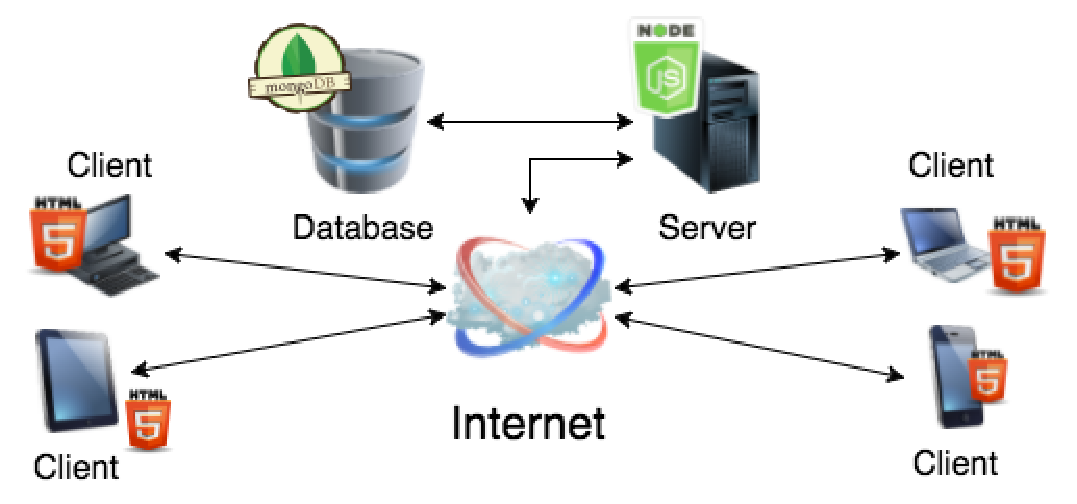
\includegraphics[scale=0.3] {figure/Architecture}}
	\caption{CrowdNote Architecture}
	\label{architecture}
\end{figure}


\subsection{The Server Component}
The server system, illustrated in Figure~\ref{server}, is composed of 3 modules: Collector, Aggregator and Player Provider.

\begin{figure}[h!]
	\centerline{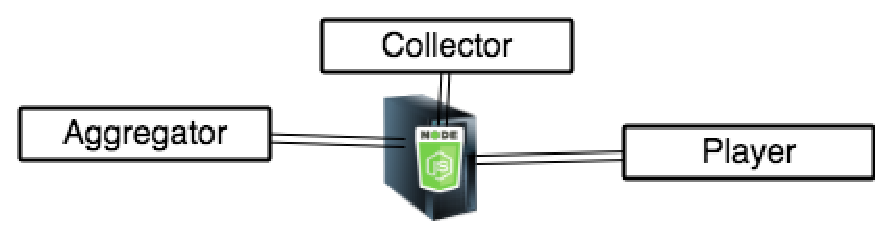
\includegraphics[scale=0.4] {figure/server}}
	\caption{Server Component}
	\label{server}
\end{figure}

\begin{itemize}

\item \textbf{Collector: } The Collector sends the jobs to the workers, receives the annotations from them, and stores the annotations into the Database.

\item \textbf{Aggregator: } Aggregator verifies, filters, groups, and processes the collected annotations of the crowd according to the rules defined for each task, and then stores the result in the Database.

\item \textbf{Player Provider: } The Player Provider sends to the client the annotations, the extra content, and the original video. Thus, the player on the client can play the enriched video synchronously.

\end{itemize}

\subsection{The Database Component}
The persistence was addressed using MongoDB, which delivers a very attractive solution to build No-SQL databases with some characteristics that meet the crowdsourcing requirements such as high write load, high availability in an unreliable environment,  easy scaling and partition, heterogeneous data into the same collection.

In this model, JSON document collections are used instead of tables, and the documents in each collection may have a different structure to store different attributes. This feature allowed the modeling of a very simple database structure, composed of 3 collections of documents, as can be seen in Figure~\ref{persistence}. It was possible because documents in the Input and Output collections can contain different fields according to the task that consumes or generates the entries.

The Video collection stores entries related to the video segments dataset, the Input collection stores the input entries to the tasks, and the Output collection stores the contributions collected from the crowd.

\begin{figure}[h]
	\centerline{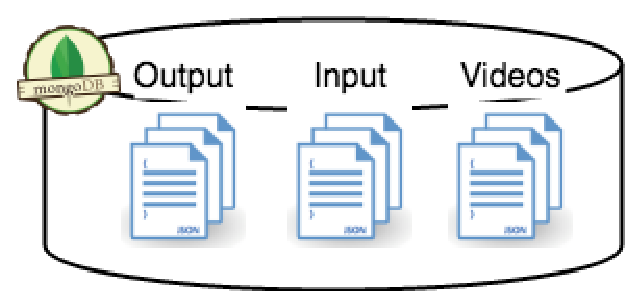
\includegraphics[scale=0.3] {figure/Persistence}}
	\caption{No-SQL Database - JSON Documents Collections}
	\label{persistence}
\end{figure}

The result of the aggregation for each task is stored in the Input collection to be used by the next task, supporting the cascading tasks approach.

\subsection{The Client Component}
The client consists of simple forms-based annotation tools and a player capable of playing video content and content synchronously. The client has been fully developed in HTML5, in the simplest way possible. For each task, a simple annotation tool was created to collect contributions.



\subsection{Workflow}
The 3 main components of CrowdNote communicate through data flows from \textbf{A} to \textbf{G}, as can be seen in the workflow in Figure~\ref{workflow}.

\begin{figure}[h]
	\centerline{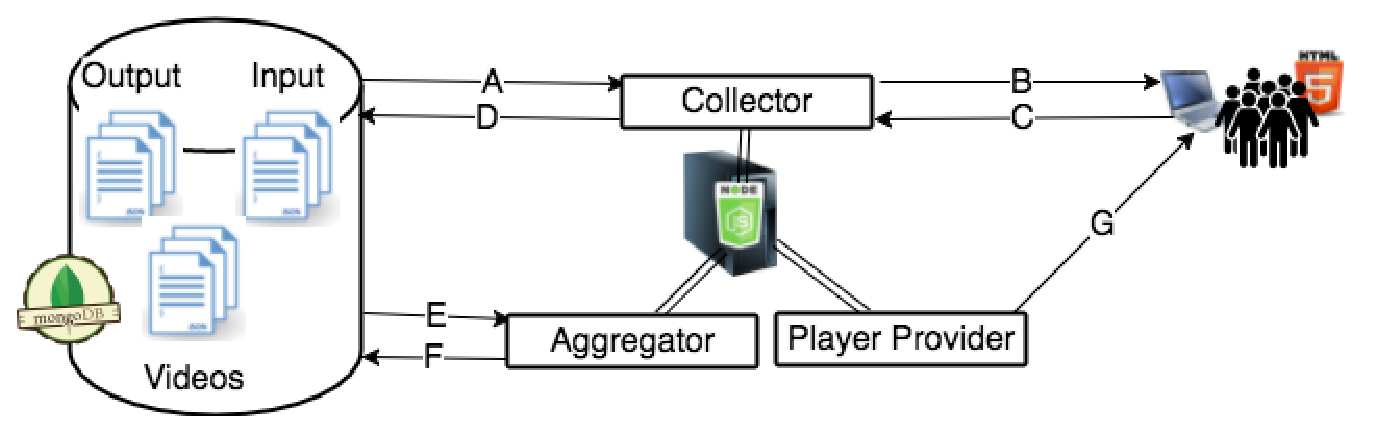
\includegraphics[scale=0.36] {figure/Workflow}}
	\caption{CrowdNote Workflow}
	\label{workflow}
\end{figure}

\begin{itemize}
\item \textbf{A:} To generate each job to be sent to a worker, the Collector receives an entry from the Input Collection and the corresponding entry from the Videos Collection.

\item \textbf{B:} The Collector sends a job to an instance of the Client, to be executed by a worker.

\item \textbf{C:} The Client sends to the Collector the annotation made by the worker for the work received.

\item \textbf{D:} The Collector stores in the Output collection the annotation collected from a worker.

\item \textbf{E:} The Aggregator receives from the Output collection all annotations collected for a given task.

\item \textbf{F:} The aggregator stores the resulting entries from the aggregation process in the Input collection so that they are supplied as input to the next task.

\item \textbf{G:} The outcome of the cascade of microtasks is sent by the Player Provider to the client so that it can play the video synchronously with the extra content.
\end{itemize}



\pagebreak

\section{Video Enrichment Instance}
	CrowdNote is an environment that can be modified to become different kinds of crowdsourcing applications based on video annotations. To create a system based on this environment is required to define the required tasks, the aggregation methods that should be applied to each task, and create the simple annotation tools for each task.

To demonstrate its working was built an instance of CrowdNote which consists of a system for video enrichment by adding extra content provided by the crowd. In this system, contributors are responsible for identifying the points of interest in the video, suggesting that the content is associated with each one, deciding the best suggestion for each point of interest, and finally deciding the best position in the video to present each content.

The extra content suggested by the crowd are images, text boxes, Wikipedia content, and Youtube videos, and the result delivered by this system is an enriched video, that consists of the original video presented synchronized with the extra content provided and selected by the crowd. 

The approach taken to achieve the complex annotation needed to enrich the videos is to cascade microtasks that collect simple annotations, instead of collecting complex annotations for each contribution. In this way, people without specialization or training can contribute to the process.


\begin{itemize}
\item \textbf{Task 1 - Identify the points of interest} in the video that should be associated with the extra content. The first microtask is to send video segments to the worker and ask him to identify in this segment something that he believes deserves to be highlighted or supplemented. The aggregation rules for this microtask are to temporarily group the annotations with a tolerance of 0.5 sec, to count and to merge similar annotations in each group, and to determine for each time group which is the predominant point of interest in the annotations.

\item \textbf{Task 2: Provide extra content suggestions} for each point of interest. In the second task, the worker receives a point of interest and should to suggest extra content related to it. This content can be a text, an image, a YouTube video or a Wikipedia page. The aggregation of the second task consists in grouping the contributions by a point of interest and joining similar contributions to avoid duplicity.

\item \textbf{Task 3: Ranking the suggested content} provided by each point of interest. In the third microtask, the worker receives a point of interest and the content suggestions for it. The contributor should choose the most appropriate content for the point presented. The aggregation rule for this task is to select the most popular content for each point of interest.
	
\item \textbf{Task 4: Determine the positions} to display the extra content associated with each point of interest. In this task, the worker receives an item that represents a point of interest and chooses the position in the video most suitable to display it. The aggregate for this task calculates the average coordinate for each item to be displayed in the video.

\end{itemize}

\pagebreak


\subsection{Cascading Microtasks}
The adopted approach consists in divide the complex annotation into simple annotations that can be collected by 
a set of simple annotation tools. Each of these simple annotations is collected by a microtask.

How is illustrated in Figure~\ref{cascading}, the input for each task is generated by the Aggregator after the previous task, except for the task 1. For this task is provided a bootstrap Input that is a list of video segments provided by the owner, that is who initiate the process. Each entry of the bootstrap input can represent a semantic block of the video. 

\begin{figure}[h!]
 \centerline{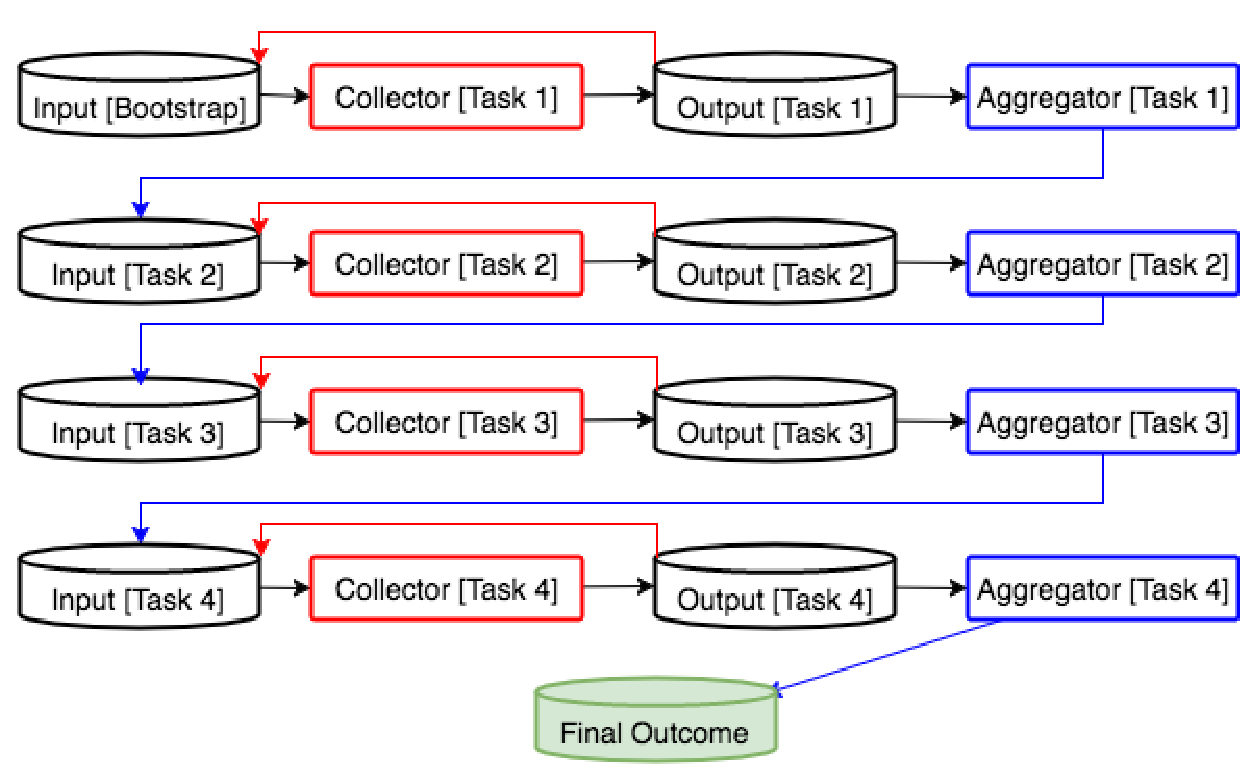
\includegraphics[scale=0.35] {figure/Cascading}}
	\caption{Cascading Microtasks}
	\label{cascading}
\end{figure}

Other applications that use CrowdNote may use different strategies to segment videos such as fixed time-length, SRT files, or even add a microtask to segment videos.
		


\subsection{Task 1}
\textbf{Identify Points of Interest:} The first annotation microtask is supported by the tool represented in Figure~\ref{task_1}, collecting identification for points of interest. In this task, the contributor receives a segment of video that should be watched, and if was found any point of interest, it should be marked and briefly described. These points of interest can be gestures, words, expressions, facts, concept, characters, events or anything that can be related to extra content.

\begin{figure}[h!]
	\centerline{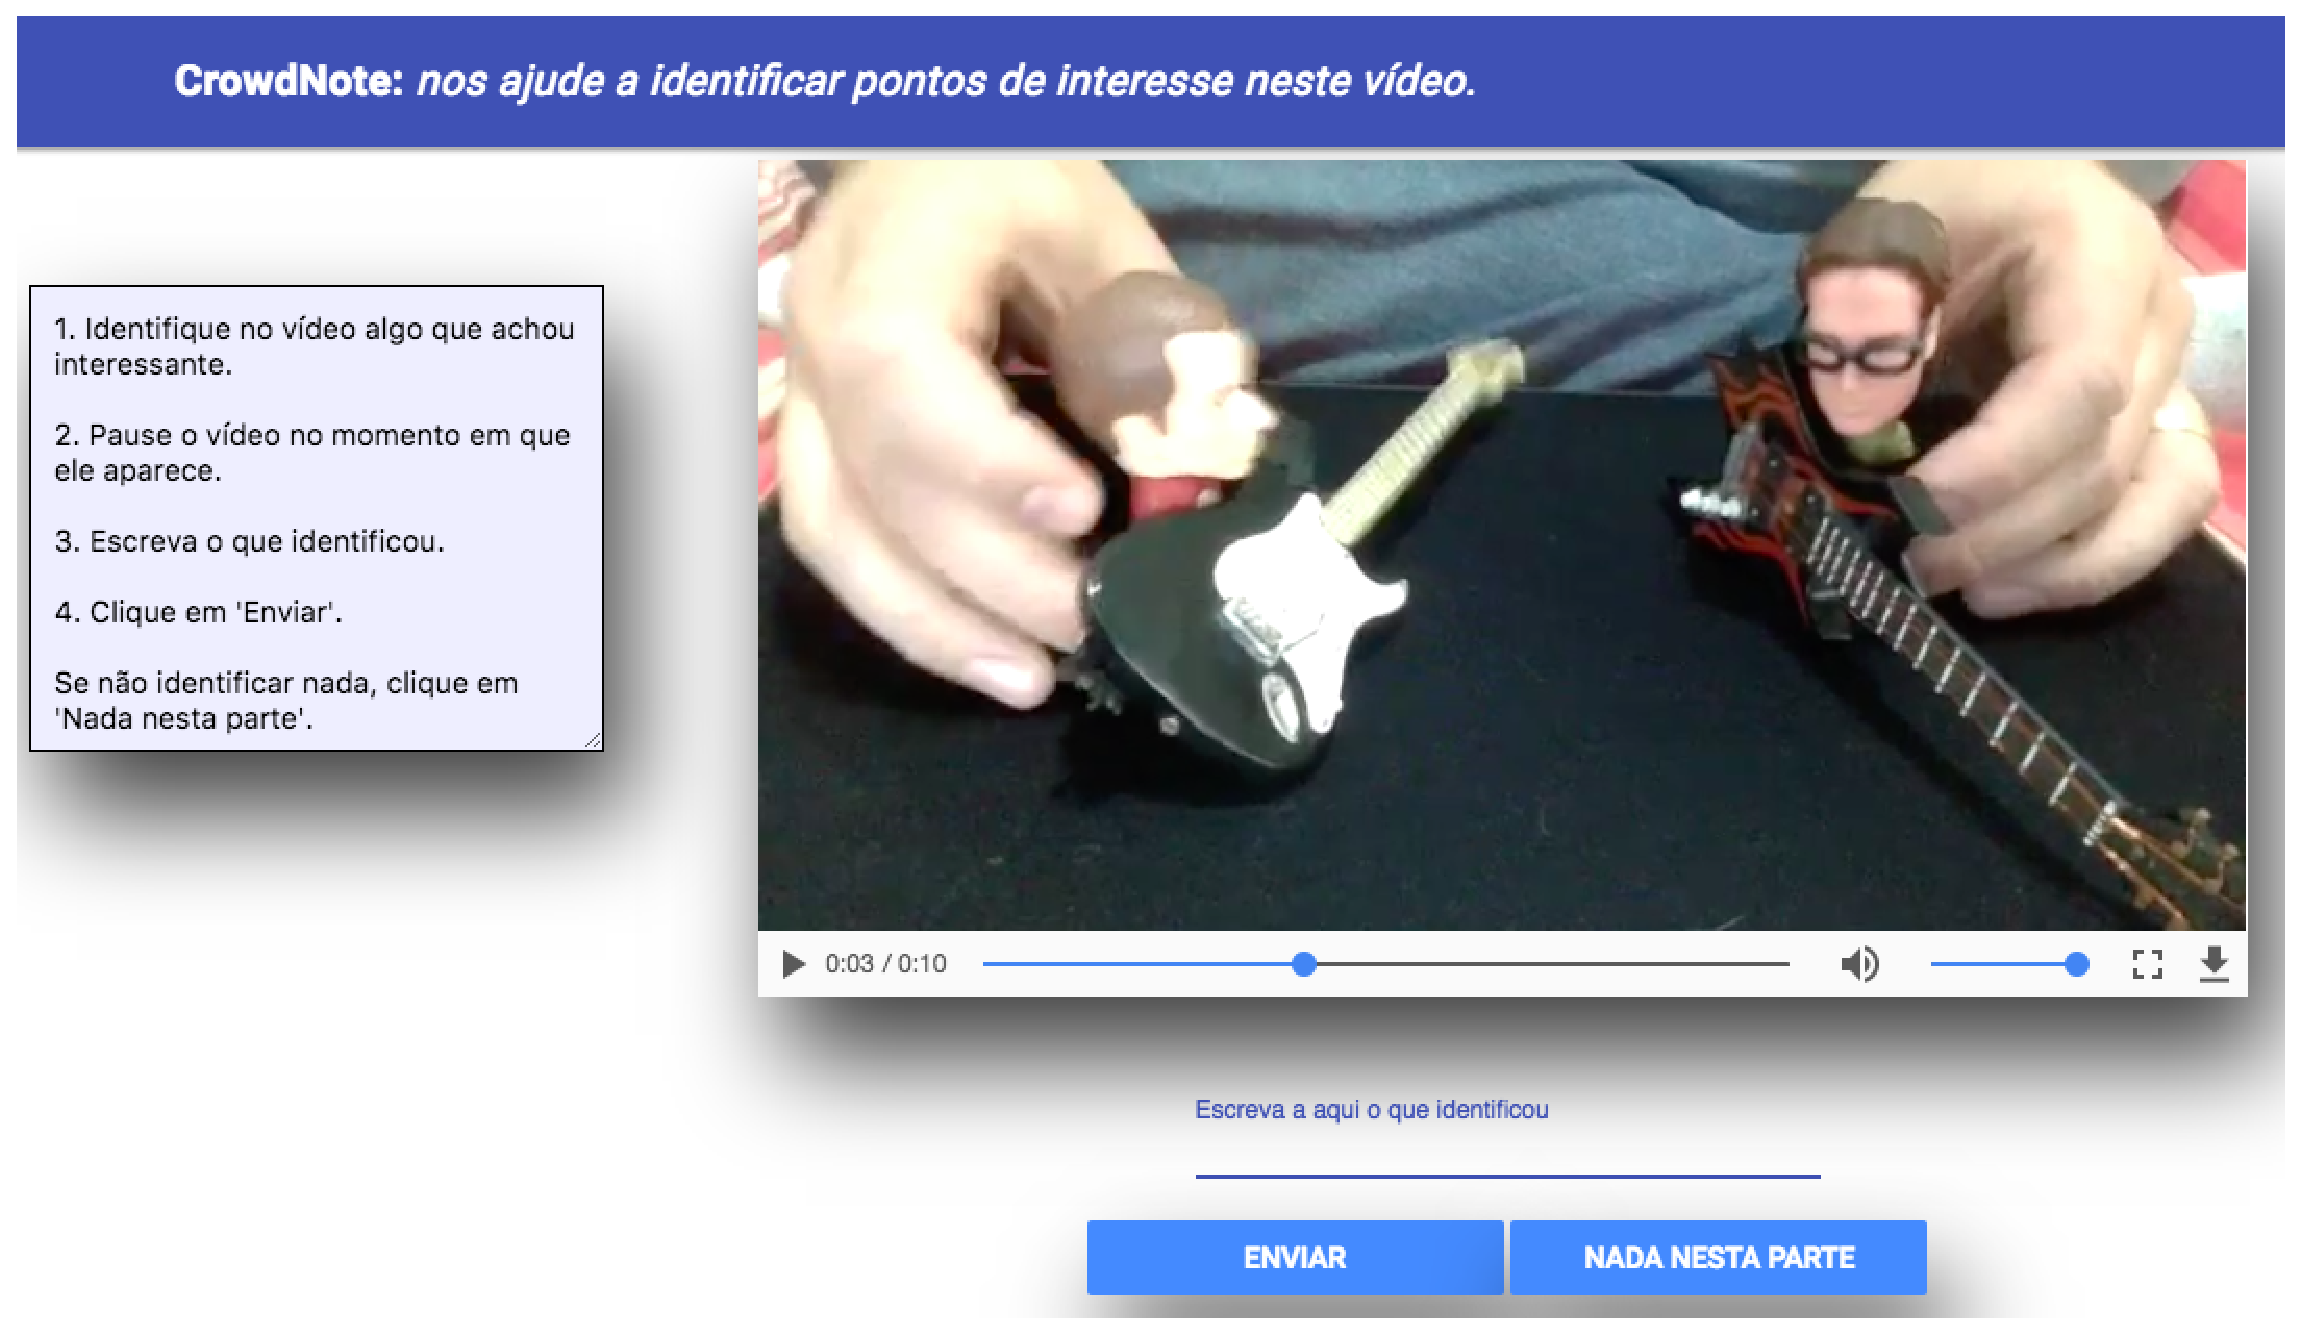
\includegraphics[scale=0.22] {figure/task_1}}
	\caption{Annotation Tool for Task 1}
	\label{task_1}
\end{figure}

\subsection{Task 2}

\textbf{Provide extra content suggestions:} The second task took as input the aggregated result from the task 1 that is a list of points of interest identified by the workers. This microtask is supported by the annotation tool represented in Figure~\ref{task_2}. This tool presents the worker a point of interest and the video segment positioned at the moment it occurs. This way, you can use video for reference and contextualization.

Through this tool, the worker can contribute by writing a text related to the point of interest, sending an image or sending a link to a YouTube video or a Wikipedia page.

\begin{figure}[h!]
	\centerline{\includegraphics[scale=0.18] {figure/task_2}}
	\caption{Annotation Tool for Task 2}
	\label{task_2}
\end{figure}

When you close the collection of contributions for this task, the Aggregator groups the content of the sender by a point of interest, and then joins the similar suggestions. In this way, a list of points of interest with a set of content suggestions for each is added to the next task, without repeated suggestions.


\subsection{Task 3}

\textbf{Ranking Suggestions:} The third task receives as input the list of points of interest, with the content suggestions for each of them. For each job, the annotation tool illustrated in Figure~\ref{task_3} shows the worker a point of interest and the video positioned at the time that point occurs. The annotation tool displays the content suggestions for that point of interest below the video, so you can browse through the content to choose the most appropriate one.

\begin{figure}[h!]
	\centerline{\includegraphics[scale=0.22] {figure/task_3}}
	\caption{Annotation Tool for Task 3}
	\label{task_3}
\end{figure}

The worker can enlarge each content to see it better, how can be seen in Figure~\ref{zoom_task_3}. In addition to playing the videos as a suggestion of content.		
		
\begin{figure}[h!]
	\centerline{\includegraphics[scale=0.18] {figure/zoom_t3}}
	\caption{Annotation Tool for Task 3 - Zoom}
	\label{zoom_task_3}
\end{figure}

The aggregation process for this task counts the votes for each content suggestion and chooses the most popular content for each point of interest.



\subsection{Task 4}

\textbf{Determine the positions:} The last task receives as input the list of points of interest and the content chosen to associate with it. For each job, the tool shown in Figure~\ref{task_4} shows the worker the video that is positioned at the time the point of interest occurs and the reference item for the content selected in the video.

The contribution to this task is to suggest the best position to present the extra content, using the annotation tool to determine this position. The tool allows the worker to change the position of the item in the video by clicking the desired point. Among the 4 microtasks, this is the fastest and easiest to perform.

\begin{figure}[h!]
	\centerline{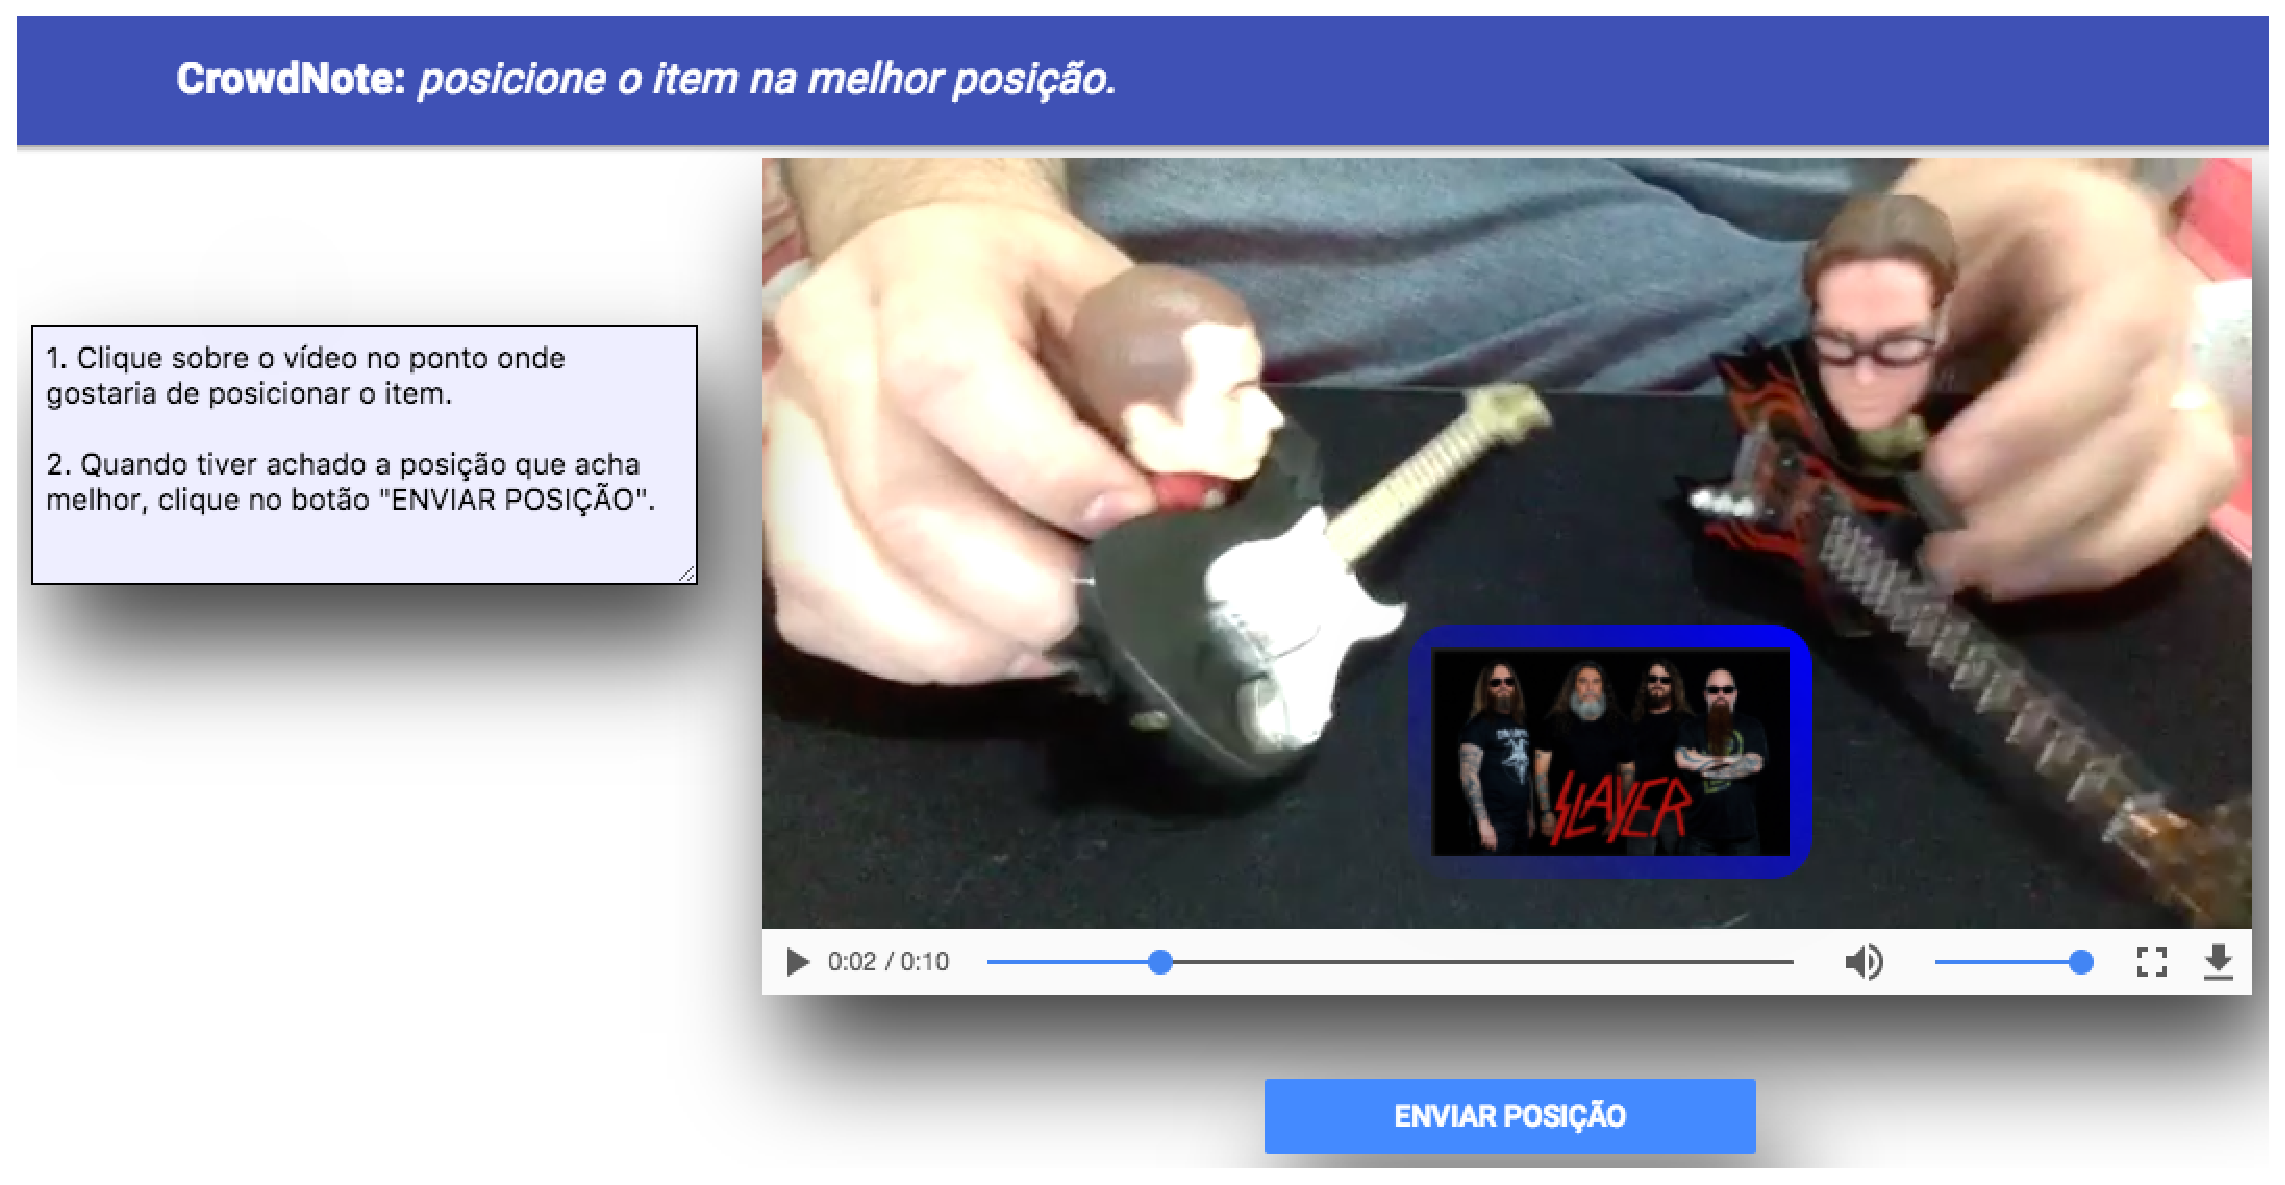
\includegraphics[scale=0.22] {figure/task_4}}
	\caption{Annotation Tool for Task 4}
	\label{task_4}
\end{figure}

Following the studies about the wisdom  of the crowd, the strategy to determine the correct position is to calculate the average coordinate of the contribution for each content \citep{GALTON1907}. In this way, the aggregation process calculates the average coordinate of the items, based on the contributions of the crowd. The result of this process is the position where each item related to a point of interest that will appear in the video.


\pagebreak

\subsection{Player}

The presentation system, shown in Figure~\ref{player}, receives the video, extra content, and necessary meta-data from the Player Provider. This system is capable of reproducing the original video synchronized with the extra content, that is displayed every time a point of interest happens in the video. Is important to remind that all extra content displayed with the video was provided, selected and positioned by the crowd.

\begin{figure}[h!]
	\centerline{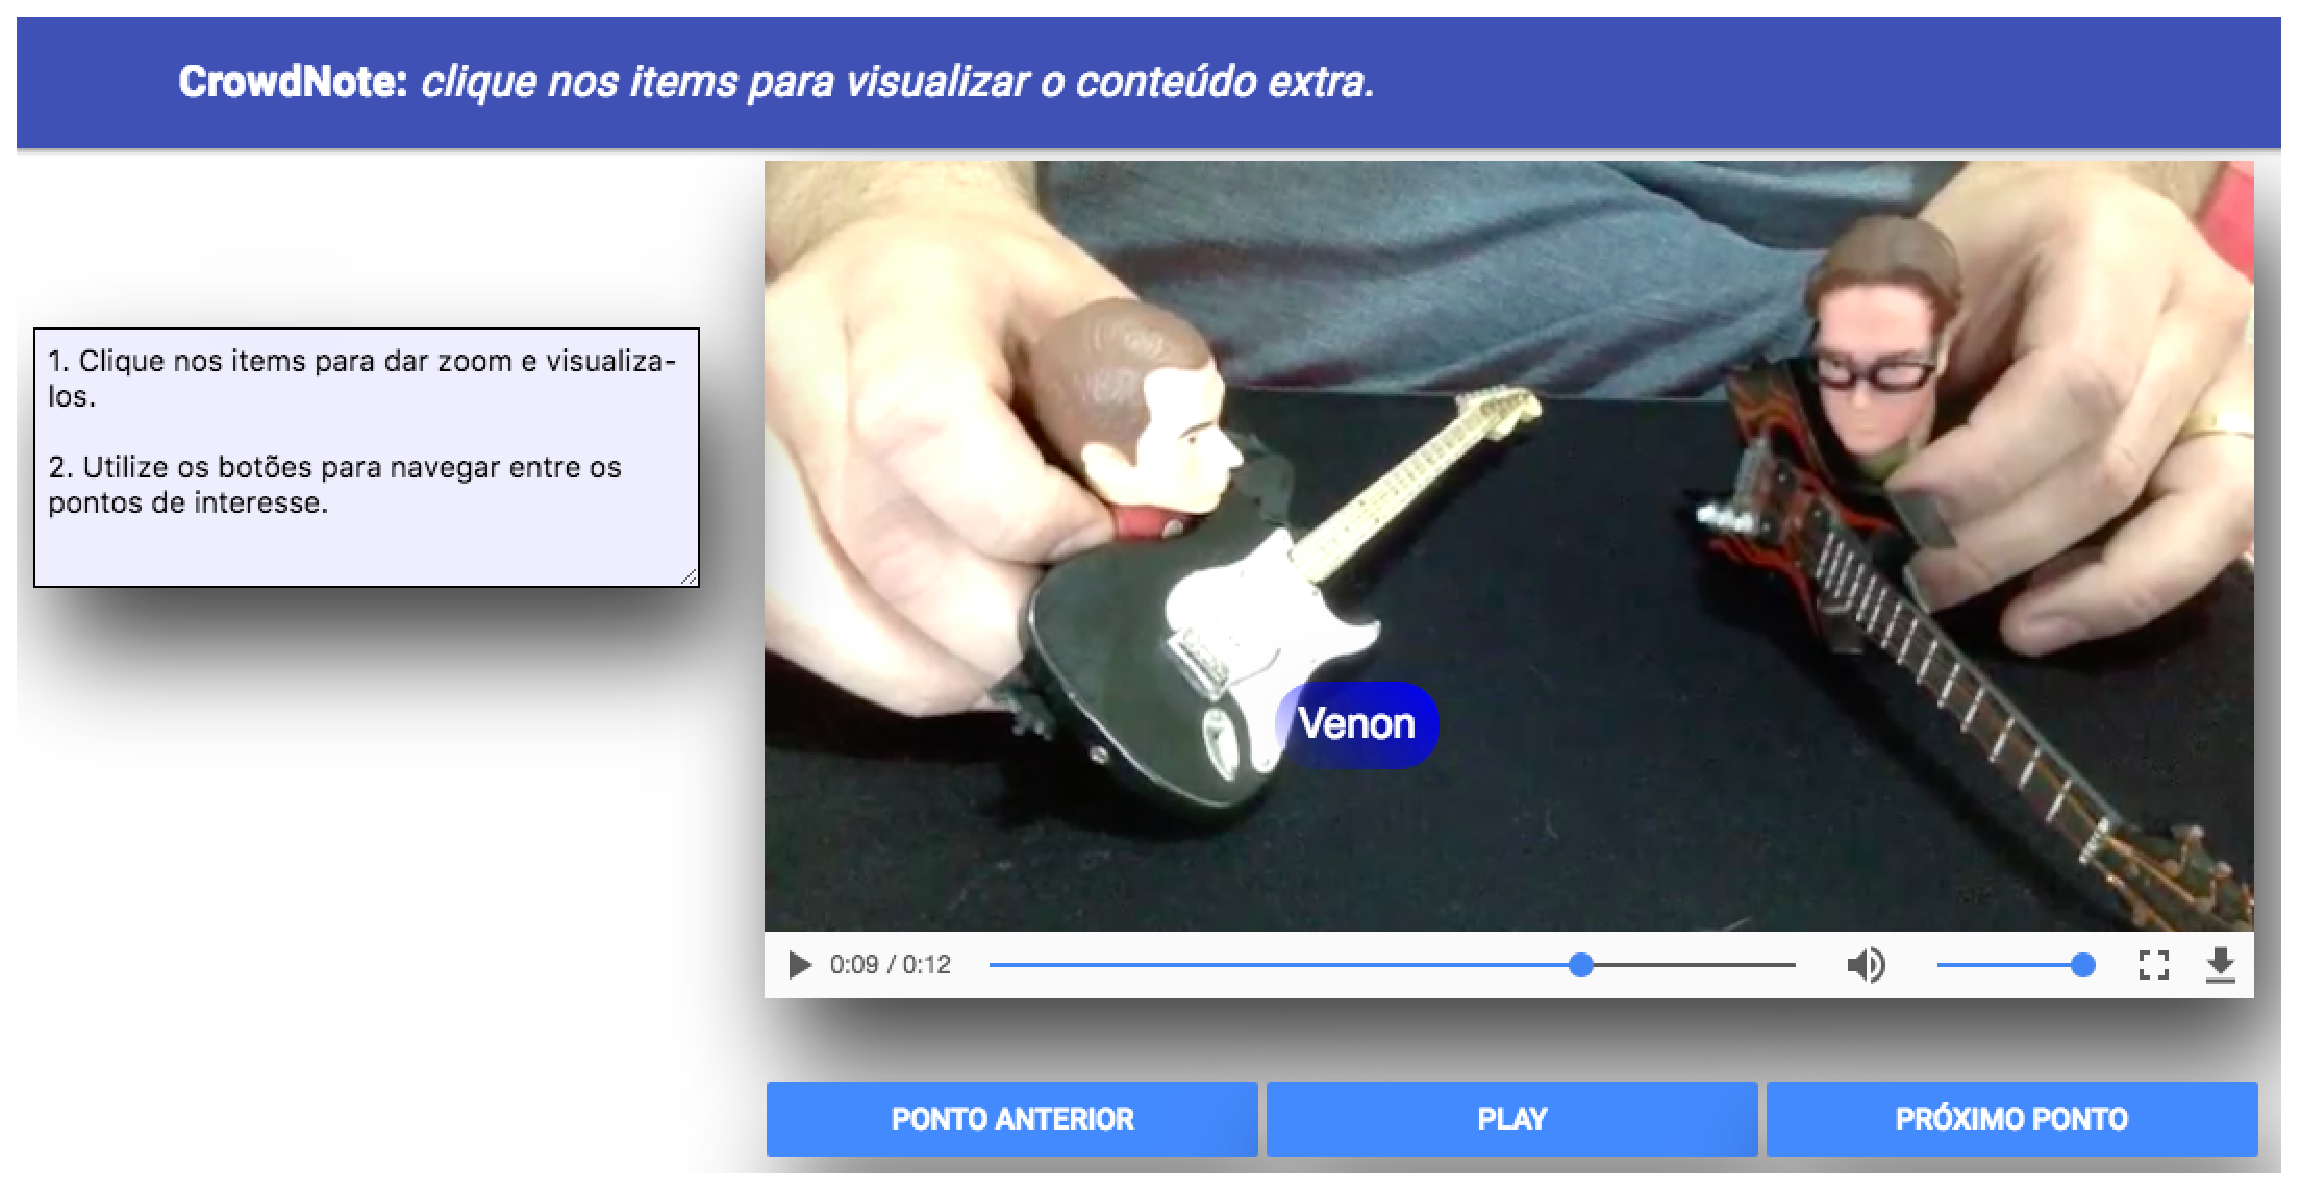
\includegraphics[scale=0.22] {figure/player}}
	\caption{Displaying an extra content item over the video}
	\label{player}
\end{figure}

When the user clicks on some extra content displayed in the video, the presentation is paused and a larger preview of the selected content is displayed in the zoom box as shown in Figure~\ref{zoom}. This system features navigation by extra-content instead the traditional timeline navigation, making available a button-bar with buttons to navigate among the extra contents.
 
\begin{figure}[h!]
	\centerline{\includegraphics[scale=0.18] {figure/zoom}}
	\caption{Displaying an extra content into a zoom modal}
	\label{zoom}
\end{figure}

	
%\section{Job Router}
%	The method used for the distribution of jobs among workers was defined according to two main criteria: 1. In each task, a worker can not contribute more than once to the same item; 2. It is desirable to obtain homogeneous coverage for items with similar amounts of contributions.

To meet the first requirement, the fingerprint of each worker is captured. This fingerprint is generated from the IP address and the signature of the Web browser. In this way, the system does not send the worker a job with an item he has already contributed.

The solution found to achieve a relatively homogeneous coverage of the items to be annotated, was adopted a routing strategy based on FIFO (first in first out) and LIFO (last in first out) structures, in accordance with the following rules:


\begin{itemize}

\item For each task, initially the items to be annotated are inserted into the entry LIFO.

\item For each job request, items are removed from the entry LIFO until an item that has not yet been annotated by the worker is found.

\item Items that have already been annotated by the worker are inserted into a temporary FIFO, which are re-entered into the entry LIFO when is found an item that still was not annotated by the worker.

\item When a worker has already annotated all the items, he is directed to a thank you page and receives no more items for that task.

\item Items taken from the entry LIFO and separated to be annotated, are inserted into the exit LIFO.

\item When the entry LIFO is empty, it is replenished by the exit LIFO, preserving an original order as far as possible.

\end{itemize}

This strategy aims to avoid that an item already annotated by a worker needs to wait until the next round is marked by another contributor. Initially, the use of a circular FIFO was considered. However, in a crowdsourcing environment, it would be very expensive to create mechanisms so that the elements already annotated by one worker would not sink until the end of the FIFO, losing the chance of being annotated by another worker in that round.

	
	
\section{Final Remarks}
	
This paper presented a method for achieving a complex media annotation by running a process workflow composed of simple annotation microtasks in a cascading arrangement. 

%Some relevant improvements were made to both the method and the framework used to support its activities.

%The contribution of this manuscript is twofold. Firstly, we have improved the cascading process proposed in [REMOVED FOR BLIND REVIEW]. Secondly, YYY


Although more studies are needed, the experiment showed in the first analysis that the cascading method based on microtasks can produce an annotated content that is coherent and comparable to the one produced by an experienced annotator. The worker's contributions were obtained from a commercial crowdsourcing environment, but with a differentiated approach in which only the resources related to the workers and none of the platform resources were used. This approach ensured that both the data set used and the data collected in the contributions were stored only in our database, not the crowdsourcing platform.


It was also observed that the concept of supervised aggregation introduced in this paper obtained positive results. This aggregation approach has proven to be interesting for improving the results of annotation tasks that receive open answers that need to be adjusted manually. A direct conclusion is that this approach can also be used to insert a human verification step at the end of certain aggregation activities.

%The diagrams introduced considerably facilitated the creation of the workflow from the production process to the case study. In addition, a specification of the dataflow in the interfaces between the components, facilitating the planning of the distribution of the works and the information that is necessary.

%The basic annotation tools distributed with the framework can be easily adapted to work with the commercial crowdsourcing platform as well as to meet the requirements of the tasks required for the experiment.

%As can be seen in Figure \ref{workers}, the workers who contributed to the experiment are scattered all over the world. This ensured a heterogeneous crowd, which contributed to the operation of aggregation methods based on the wisdom theory of the crowds.
%\begin{figure}[h]
%	\centerline{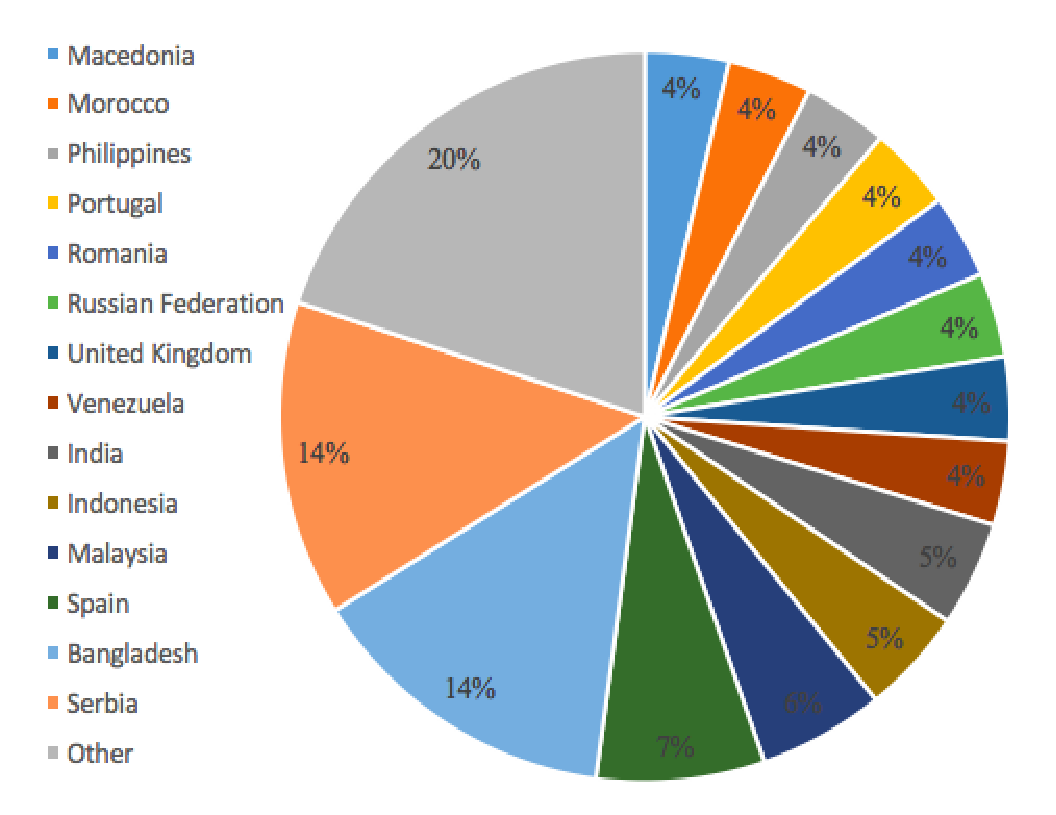
\includegraphics[scale=0.4] {figure/workers_2}}
%	\caption{Workers distribution through the world.}
%	\label{workers}
%\end{figure}

The video enrichment process has been able to produce an interactive multimedia presentation from a simple raw video through a crowdsourcing approach. This leads to the conclusion that the updated method presented is appropriate to guide this type of project that aims to generate complex media annotations.

\subsection{Issues}
Some issues were detected in relation to the collection process. About 20\% of the contributions cannot be used because they did not meet the desired specifications or because they had invalid or malicious content. This showed that it is necessary to insert in the annotation tools some resources that induce workers to provide valid contributions. It also alerted us to the importance of giving workers clearer instructions on how to properly perform tasks.

In fact, it drew attention to the need to define criteria for the evaluation of instructions given to workers. Also it brings the discussion about the need for a research on whether textual instructions are really sufficient to perform any simple annotation microtasking.

\subsection{Crowds Comparison Experiment}
Another relevant discussion from the observations of the results concerns the extent to which the composition of the crowd can influence the outcome.

To better understand, the experiment conducted will be replicated in different scenarios:
\begin{itemize}
\item Increasing the salary of workers;
\item Choosing different contracted groups;
\item Choosing only the best workers;
\item Using a closed group with volunteers;
\item Using a group familiar with the subject treated in the video;
%\item Using a group of natives in the English language.
\end{itemize}

\pagebreak

\subsection{Next Steps}

This work is constantly improving on three different fronts: improvement of the method, improvement of the system, use of the method in different scenarios and applications.

Regarding the method, the next steps include the formalization of the aggregation process, defining specific flows for automatic, supervised and manual models.

New annotation tools are being designed for the structure, which can be adapted for more tasks. In addition, a wizard is being designed to guide the creation of complex media annotation projects based on the method presented.

Some experiments are being prepared to be carried out, some of which seem especially promising:
\begin{itemize}
\item Multisensorial video annotation for mulsemedia applications.
\item Gesture segmentation in signal language video datasets.
\item Semantic approximation of idiomatic expressions in automatic translations.
\item Crowdsourcing  creation of learning object.
\end{itemize}


\begin{acks}
%Removed for double-blind review.
	The authors would like to thank the "Funda\c c\~ ao de Amparo \`a Pesquisa e Inova\c c\~ ao do Esp\'irito Santo" (FAPES) and "Coordena\c c\~ ao de Aperfei\c coamento de Pessoal de N\'ivel Superior" (CAPES).
\end{acks}

\bibliographystyle{ACM-Reference-Format}
\bibliography{refs} 

\end{document}
